% Template for Cogsci submission with R Markdown

% Stuff changed from original Markdown PLOS Template
\documentclass[10pt, letterpaper]{article}

\usepackage{cogsci}
\usepackage{pslatex}
\usepackage{float}
\usepackage{caption}

% amsmath package, useful for mathematical formulas
\usepackage{amsmath}

% amssymb package, useful for mathematical symbols
\usepackage{amssymb}

% hyperref package, useful for hyperlinks
\usepackage{hyperref}

% graphicx package, useful for including eps and pdf graphics
% include graphics with the command \includegraphics
\usepackage{graphicx}

% Sweave(-like)
\usepackage{fancyvrb}
\DefineVerbatimEnvironment{Sinput}{Verbatim}{fontshape=sl}
\DefineVerbatimEnvironment{Soutput}{Verbatim}{}
\DefineVerbatimEnvironment{Scode}{Verbatim}{fontshape=sl}
\newenvironment{Schunk}{}{}
\DefineVerbatimEnvironment{Code}{Verbatim}{}
\DefineVerbatimEnvironment{CodeInput}{Verbatim}{fontshape=sl}
\DefineVerbatimEnvironment{CodeOutput}{Verbatim}{}
\newenvironment{CodeChunk}{}{}

% cite package, to clean up citations in the main text. Do not remove.
\usepackage{cite}

\usepackage{color}

% Use doublespacing - comment out for single spacing
%\usepackage{setspace}
%\doublespacing


% % Text layout
% \topmargin 0.0cm
% \oddsidemargin 0.5cm
% \evensidemargin 0.5cm
% \textwidth 16cm
% \textheight 21cm

\title{Children's understanding of simple polite markers}


\author{{\large \bf } \\ \texttt{} \\  \\}

\begin{document}

\maketitle

\begin{abstract}
Here we show that, with an improvement over the age of 2 to 4 years,
English-speaking preschool children understand implications of simple
polite markers: They understand that it is more \emph{polite} and
\emph{nicer} to say ``please'' and ``can you \textasciitilde{}'' when
making requests, and that the use of these polite markers indicates that
the speaker is more socially likeable and is more likely to gain
compliance from their conversational partners.

\textbf{Keywords:}
Politeness, pragmatic development, online experiment
\end{abstract}

\section{Introduction}\label{introduction}

As adults, we use polite speech all the time.

Children produce polite speech early on.

Less work has looked at children's comprehension of polite speech.

For example, Nippold, Leonard, \& Anastopoulos (1982) looked at\ldots{}

In this current work, we sought to test what 2- to 4-year-old children
understand about polite speech. Specifically, we asked: (1) whether
children can reason about which speaker is being more ``polite'' or
``rude'' (or ``nice'' or ``mean'') based on their use of polite markers;
(2) whether they understand possible social consequences of being polite
or impolite; and (3) how this reasoning may change across development.

Across three Experiments, we presented stories about speakers who
decided to speak politely (e.g., ``Please pour me more water'') or
impolitely (e.g., ``Pour me more water'') and asked child participants
to compare between the two speakers. In Experiment 1 and 2, we found
that 3- to 4-year-old children were able to reason that a speaker who
used polite markers was more polite and nicer than a speaker who did
not, and that the polite speaker is more socially likeable and is more
likely to gain what they want, given facial expression and prosodic
cues. In Experiment 3, we recruited two samples (one from a local
nursery school and the other from an online platform) and found that
children were able to reason correctly about polite speech even when the
supportive facial and prosodic cues were removed, and this reasoning
improves from 2 to 4 years of age.

\section{Experiment 1}\label{experiment-1}

In Experiment 1, we tested whether 3- to 4-year-old children were able
to understand implications of using simple polite markers, based on not
only linguistic cues of interest (whether the speaker says ``please,''
``can you''), but also extra cues that they might need (facial
expressions and prosodic cues). Thus, we asked children to compare
between speakers who used polite markers with a kind voice and facial
expression versus speakers who did not use polite markers and spoke with
a mean, angry voice and facial expression.

\subsection{Methods}\label{methods}

\subsubsection{Participants}\label{participants}

3-year-old (\(n=\) 20; 12 F, \(M_{age}\) = 3.61 years, \(SD_{age}\) =
0.22) and 4-year-old children (\(n=\) 18; 6 F, \(M_{age}\) = 4.38 years,
\(SD_{age}\) = 0.25) were recruited from a local preschool. An
additional 3 children were tested but excluded due to failure on the
practice questions (\(n=\) 2) or completion of fewer than half of the
test trials (\(n=\) 1).

\subsubsection{Stimuli}\label{stimuli}

\subsubsection{Procedure}\label{procedure}

The experimenter presented to the child a storybook with a total of
thirteen stories about different characters. In the \emph{practice}
phase, the child heard a story with one clearly mean character
(\emph{Drew kicked Carol}) and one clearly nice character (\emph{Graham
gave Carol a gift}). After a reminder of what each character did, the
experimenter asked the participant: \emph{Which one was being meaner?}
and \emph{Which one was being nicer?} If the child answered the question
wrong the first time, the experimenter read the story one more time,
saying, ``Let's think about the story one more time.'' Only children who
correctly answered both questions in the first or second attempt were
included in the analyses.

In the \emph{test} phase, the child heard twelve stories, in each of
which they saw one speaker who decided to speak politely (\emph{Jean
wanted more water in her cup. Jean said to Fred, ``Please pour me more
water''}) and another speaker who spoke impolitely (\emph{Suzy also
wanted more water in her cup. Suzy said to Fred, ``Pour me more
water.''}). After a reminder about what each speaker said, the child was
asked a total of two questions. For the first question, the experimenter
asked one out of four possible questions: ``Which one was being more
polite {[}more rude/nicer/meaner{]}?'' For the second question, the
experimenter either asked about play partner choice (\emph{Which one
would you rather play with?}) or likelihood of compliance (e.g.,
\emph{Which one will Fred give water to?}). The order of story types and
question types was counterbalanced.

\subsection{Results and Discussion}\label{results-and-discussion}

\begin{CodeChunk}
\captionsetup{width=0.8\textwidth}\begin{figure*}[h]

{\centering 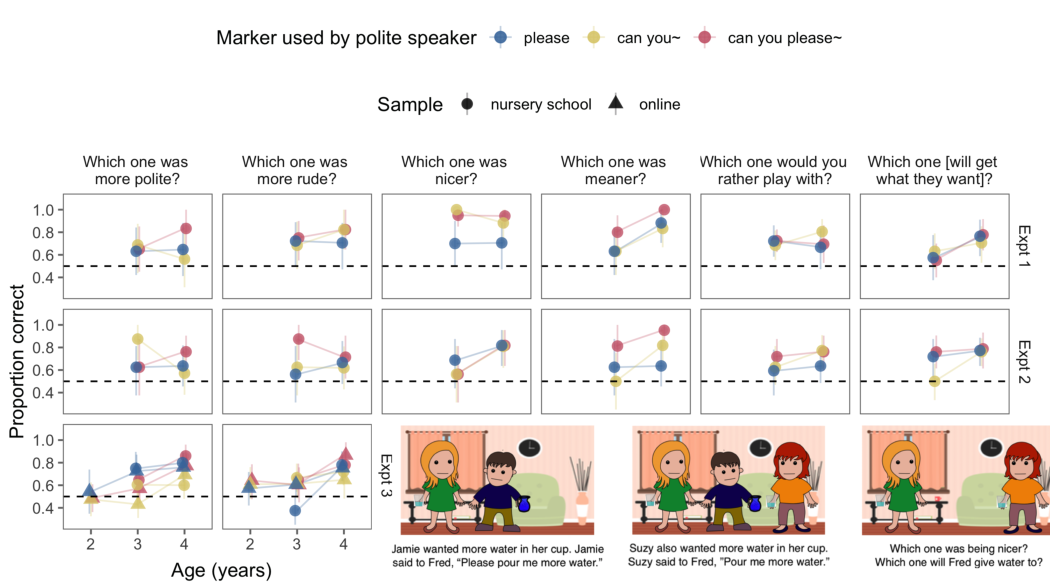
\includegraphics{figs/fig_results_placement-1} 

}

\caption[Proportion of correct responses to questions comparing between a speaker who used a polite marker (indicated at the top of each column) versus a speaker who did not]{Proportion of correct responses to questions comparing between a speaker who used a polite marker (indicated at the top of each column) versus a speaker who did not. Data are binned into one-year age groups for visualization purposes (all analyses are conducted on continuous data). Different colors represent responses from different Experiments (see legend at the top). Rows represent different questions asked (indicated on the right). Dashed line represents chance level at 50\% (i.e., if participant were guessing at random).}\label{fig:fig_results_placement}
\end{figure*}
\end{CodeChunk}

In sum, in Experiment 1, we confirmed that children were able to use
some combination of cues (markers, prosody and facial expressions) to
politeness to reason about which speaker is nicer/meaner or more
polite/rude, and which speaker is more likely to be a better play
partner and to have their needs met. But in this initial task, the
experimenter produced the utterances and was not blind to the condition,
which could have biased her presentation of the stories and therefore
participants' performances. In Experiment 2, we presented pre-recorded
voiceovers for speakers' utterances to address this concern.

\section{Experiment 2}\label{experiment-2}

\subsection{Methods}\label{methods-1}

\subsubsection{Participants}\label{participants-1}

\subsubsection{Stimuli}\label{stimuli-1}

\subsubsection{Procedure}\label{procedure-1}

\subsection{Results and Discussion}\label{results-and-discussion-1}

\section{Experiment 3}\label{experiment-3}

\subsection{Methods}\label{methods-2}

\subsubsection{Participants}\label{participants-2}

\subsubsection{Stimuli}\label{stimuli-2}

\subsubsection{Procedure}\label{procedure-2}

\subsection{Results and Discussion}\label{results-and-discussion-2}

\section{General Discussion}\label{general-discussion}

\section{References}\label{references}

\setlength{\parindent}{-0.1in} \setlength{\leftskip}{0.125in} \noindent

\hypertarget{refs}{}
\hypertarget{ref-nippold1982}{}
Nippold, M. A., Leonard, L. B., \& Anastopoulos, A. (1982). Development
in the use and understanding of polite forms in children. \emph{Journal
of Speech, Language, and Hearing Research}, \emph{25}(2), 193--202.

\end{document}
